\chapter{Process Automation}

After doing a domain analysis, we will execute the process. 

\begin{enumerate}
    \item Create an executable BPMN model in Signavio Workflow Accelerator. See~\cref{fig:bpmnModel}. 
    \item Create a functional application that supports the BPMN model using the Signavio Workflow Accelerator. See~\cref{fig:bpmnDecision}. 
    \item Create forms for BPMN activities. See~\cref{fig:bpmnForm}. 
    \item Execute the BPMN model. One happy flow, one unhappy flow. See~\cref{fig:bpmnExecution1}, and ~\cref{fig:bpmnExecution2}. 
    \item Create one meaningful report in the Analytics section. ~\cref{fig:bpmnReport}. 
    \item Demonstrate your results in a presentation. See~\cref{sec:presentation}. 
\end{enumerate}

As an example, we used models created by Martin Kutiš and Vladimír Vlk in the 2019 MI-MEP course~\cite{kutisvlk2019}. 

\section{Process Design}

\begin{figure}[h]\centering
	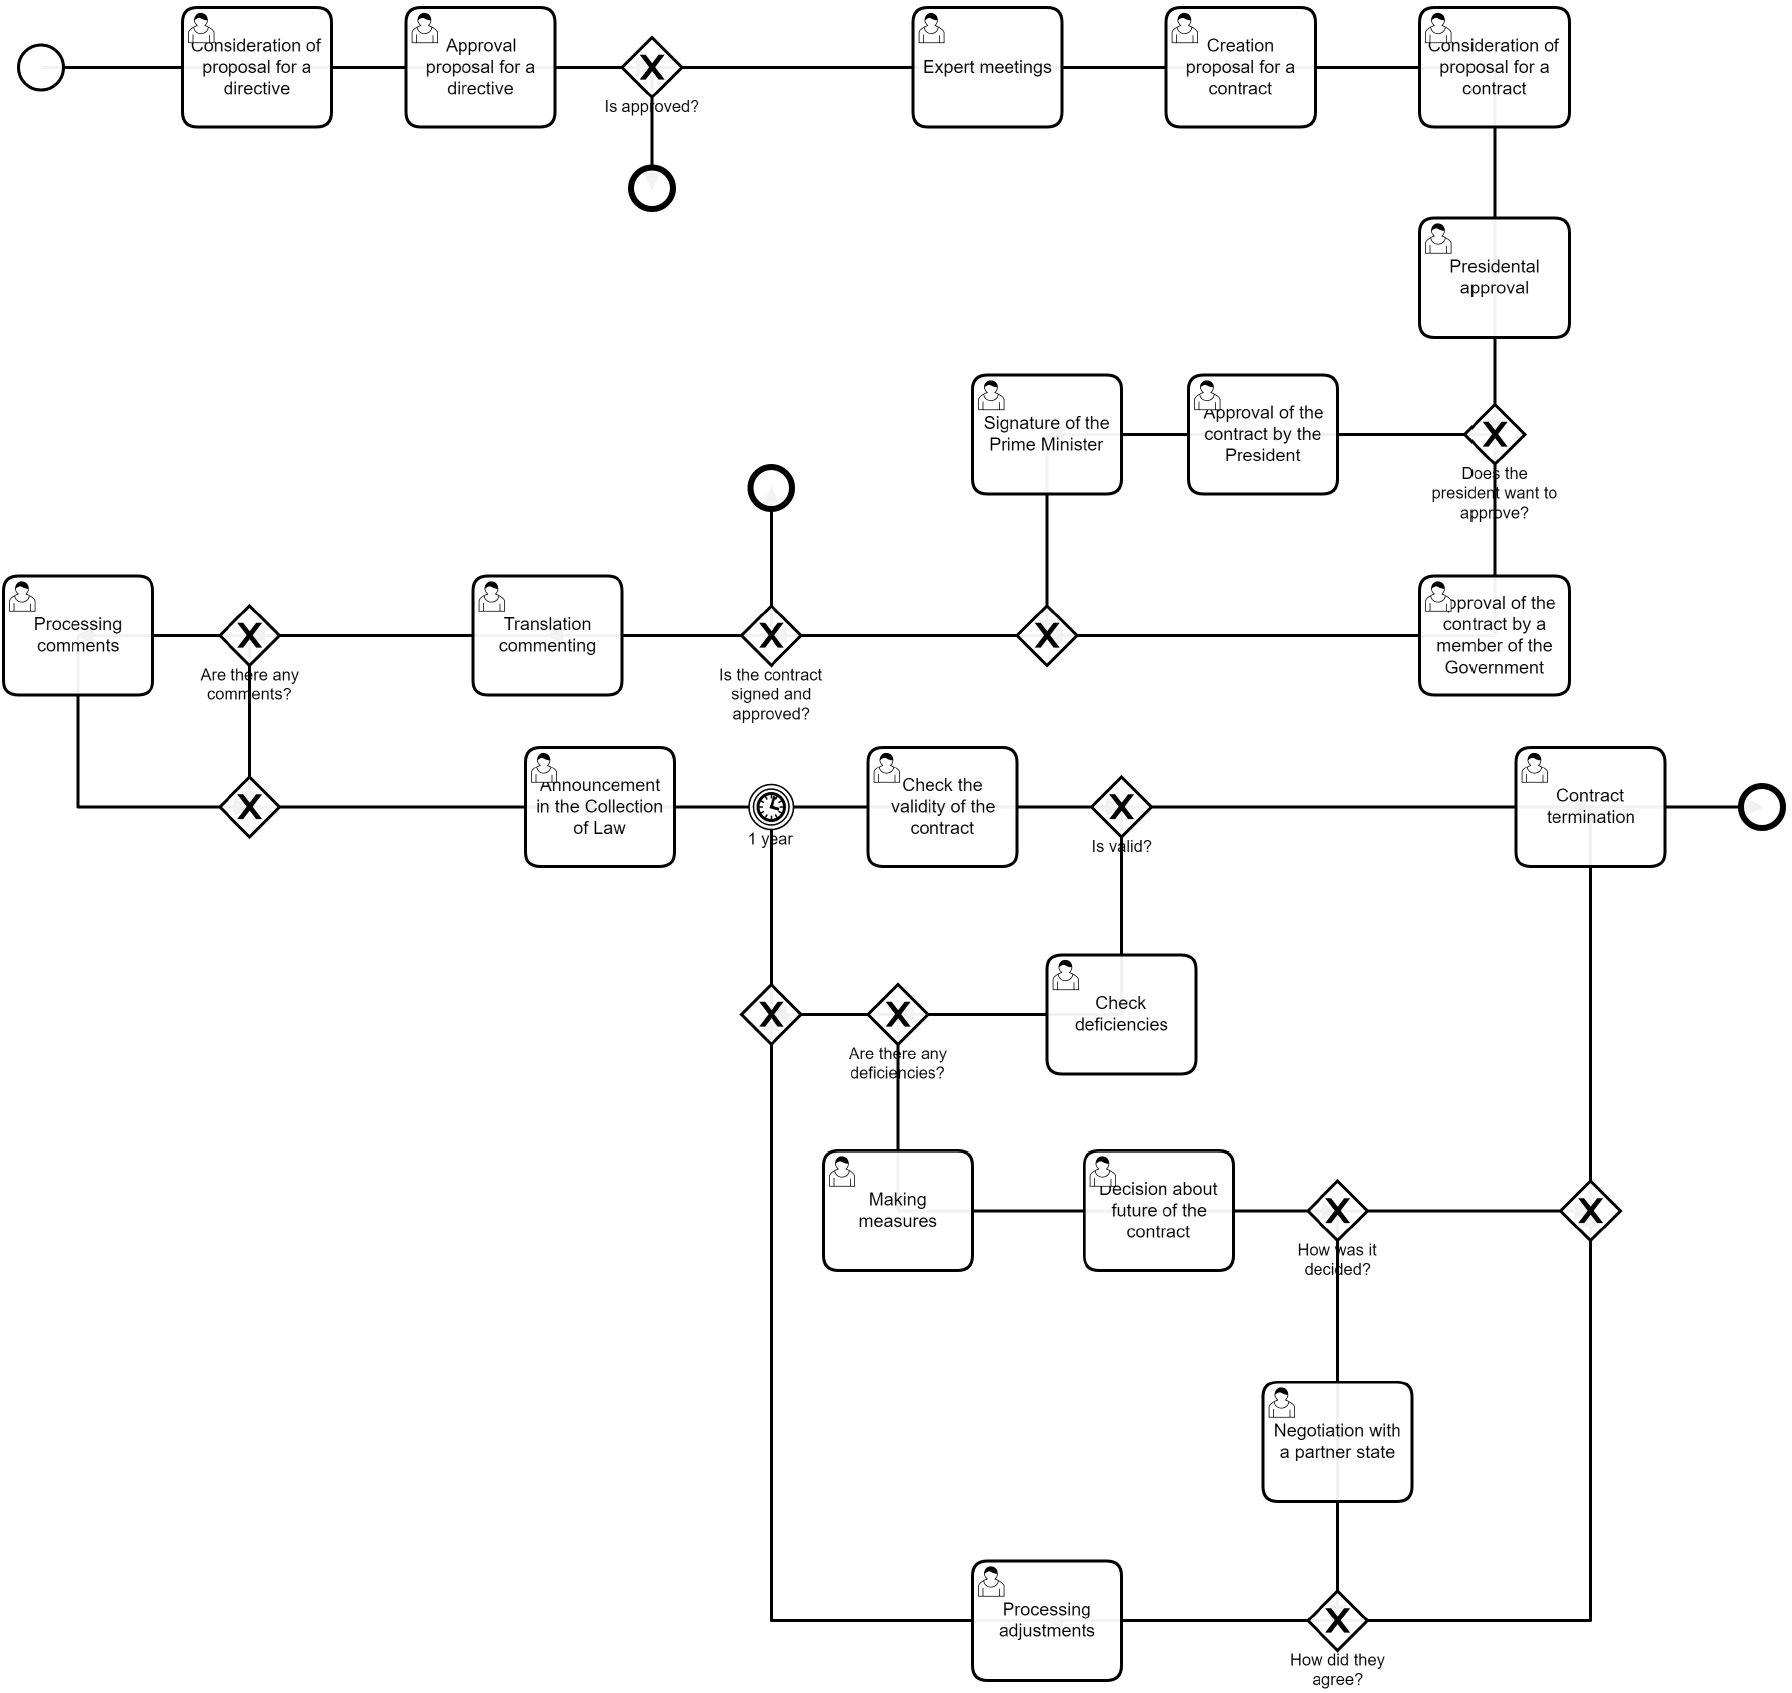
\includegraphics[width=\textwidth]{pic/BPMNModel}
	\caption{An Executable BPMN Process Model~\cite{kutisvlk2019}}
	\label{fig:bpmnModel}
\end{figure}

\begin{figure}[h]\centering
	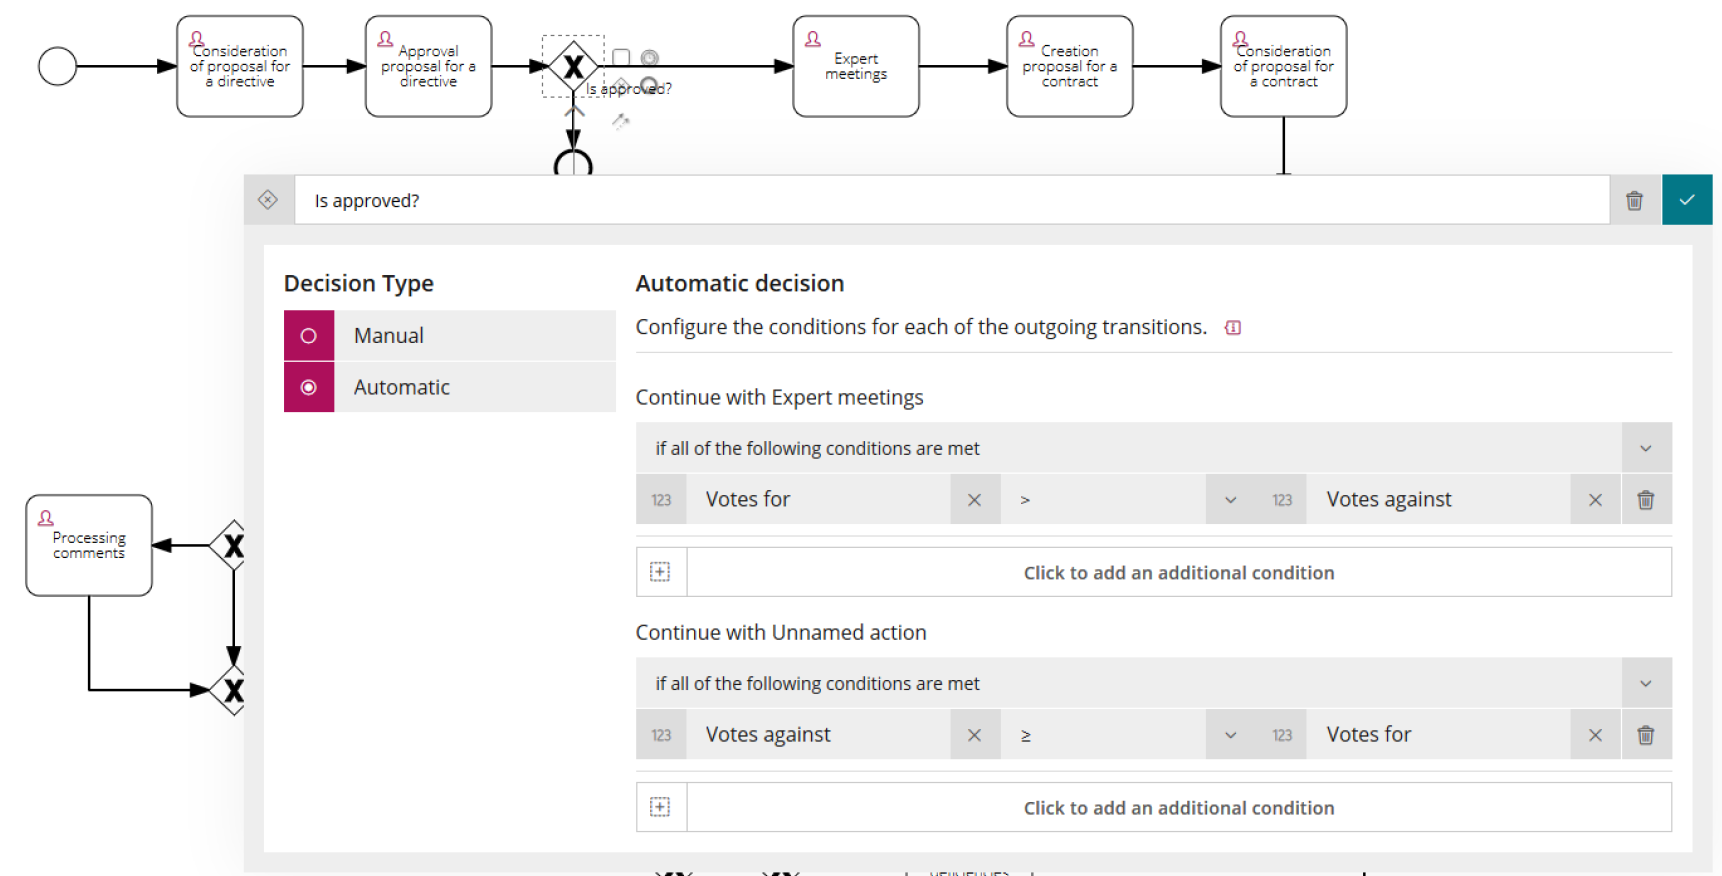
\includegraphics[width=\textwidth]{pic/BPMNDecision}
	\caption{An Executable BPMN Process Model Gateway~\cite{kutisvlk2019}}
	\label{fig:bpmnDecision}
\end{figure}

\begin{figure}[h]\centering
	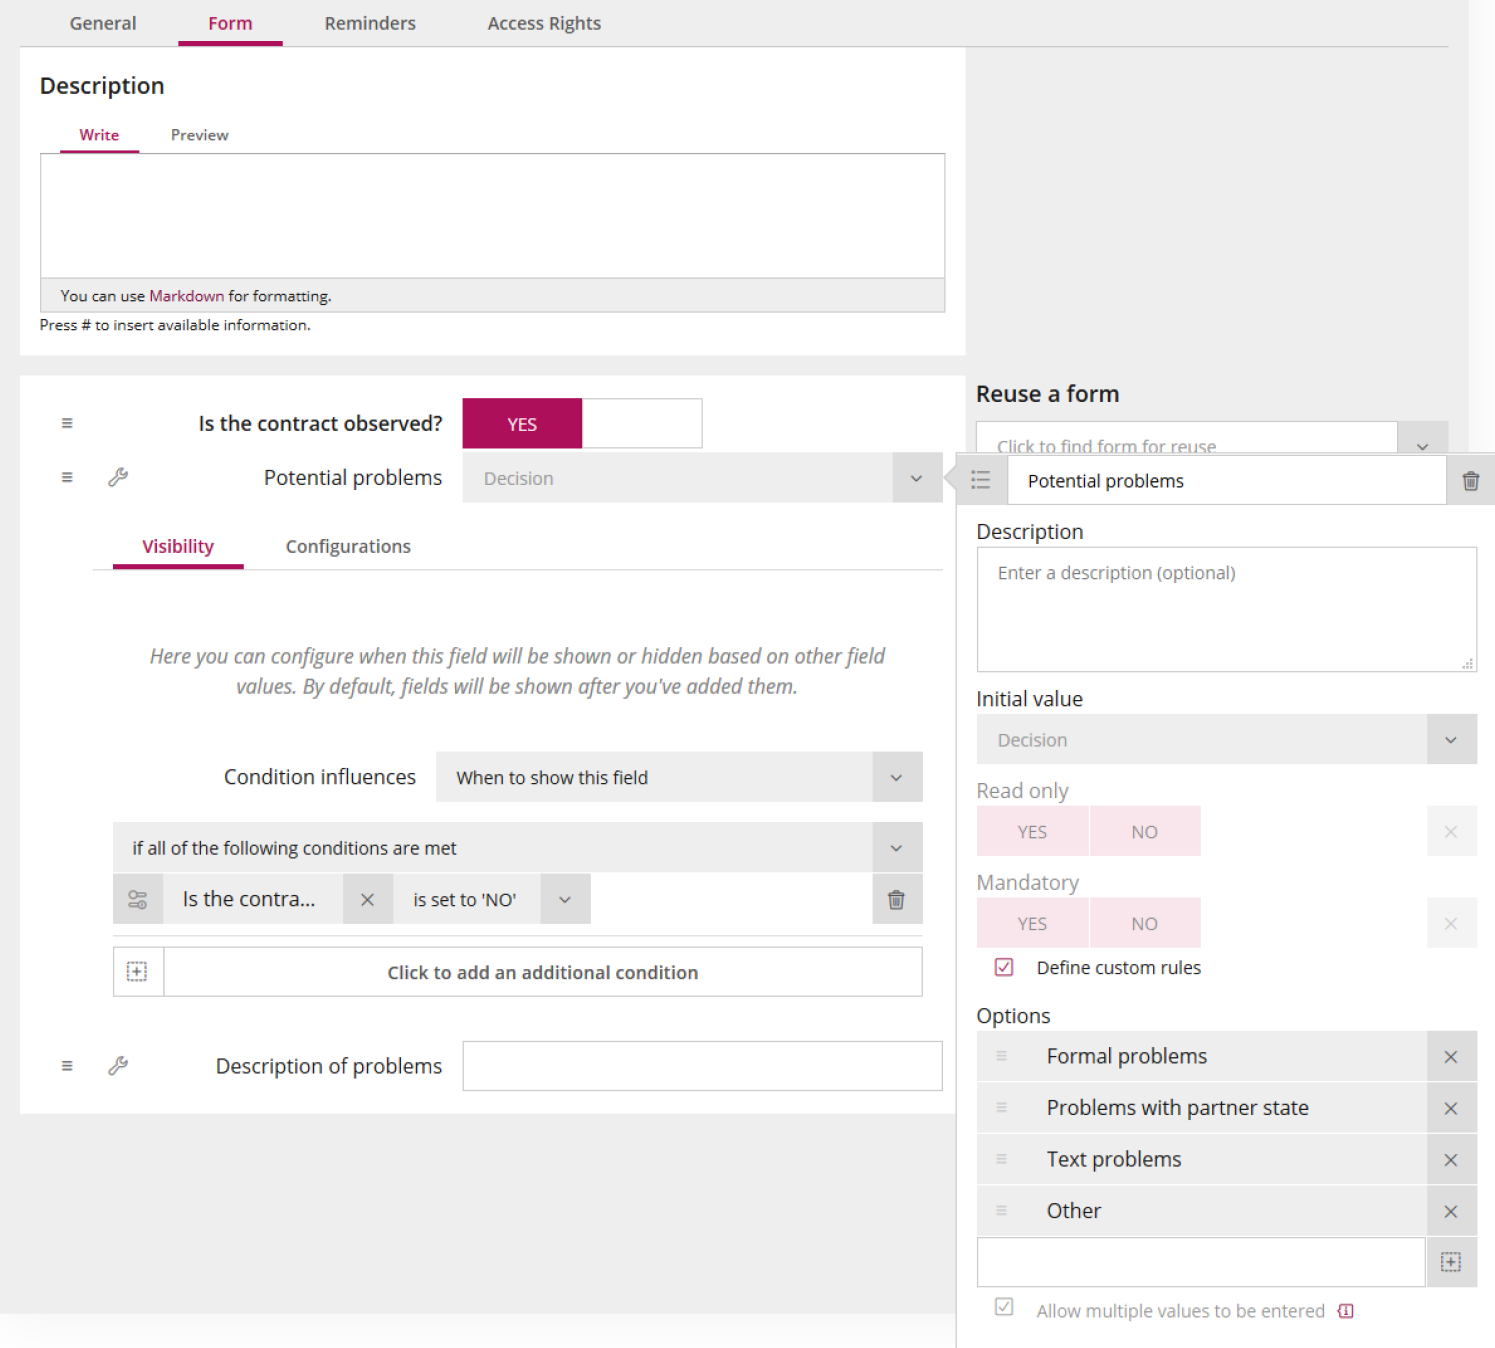
\includegraphics[width=\textwidth]{pic/BPMNForm}
	\caption{An Executable BPMN Process Model Forms~\cite{kutisvlk2019}}
	\label{fig:bpmnForm}
\end{figure}

\section{Process Execution}

Include all the important execution steps here. 

\begin{figure}[h]\centering
	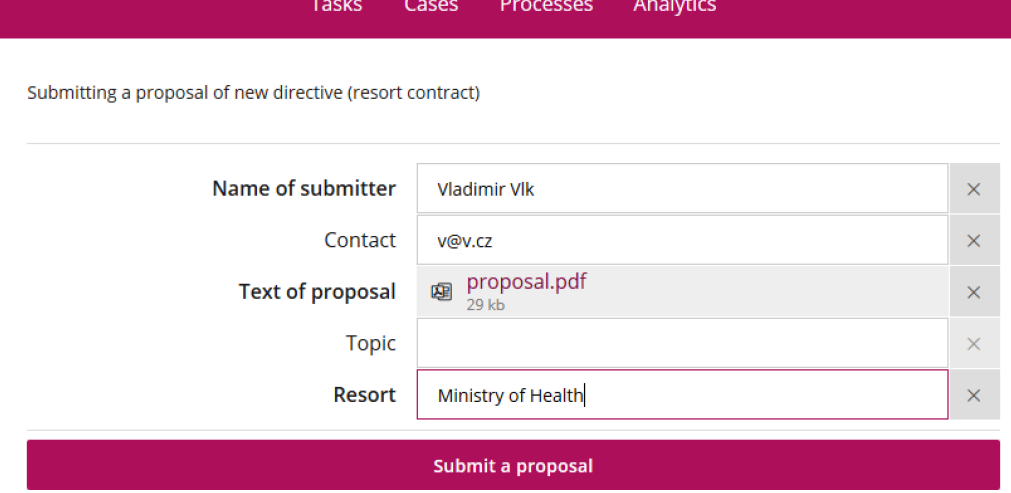
\includegraphics[width=\textwidth]{pic/BPMNExecution1}
	\caption{A BPMN Process Execution~\cite{kutisvlk2019}}
	\label{fig:bpmnExecution1}
\end{figure}

\begin{figure}[h]\centering
	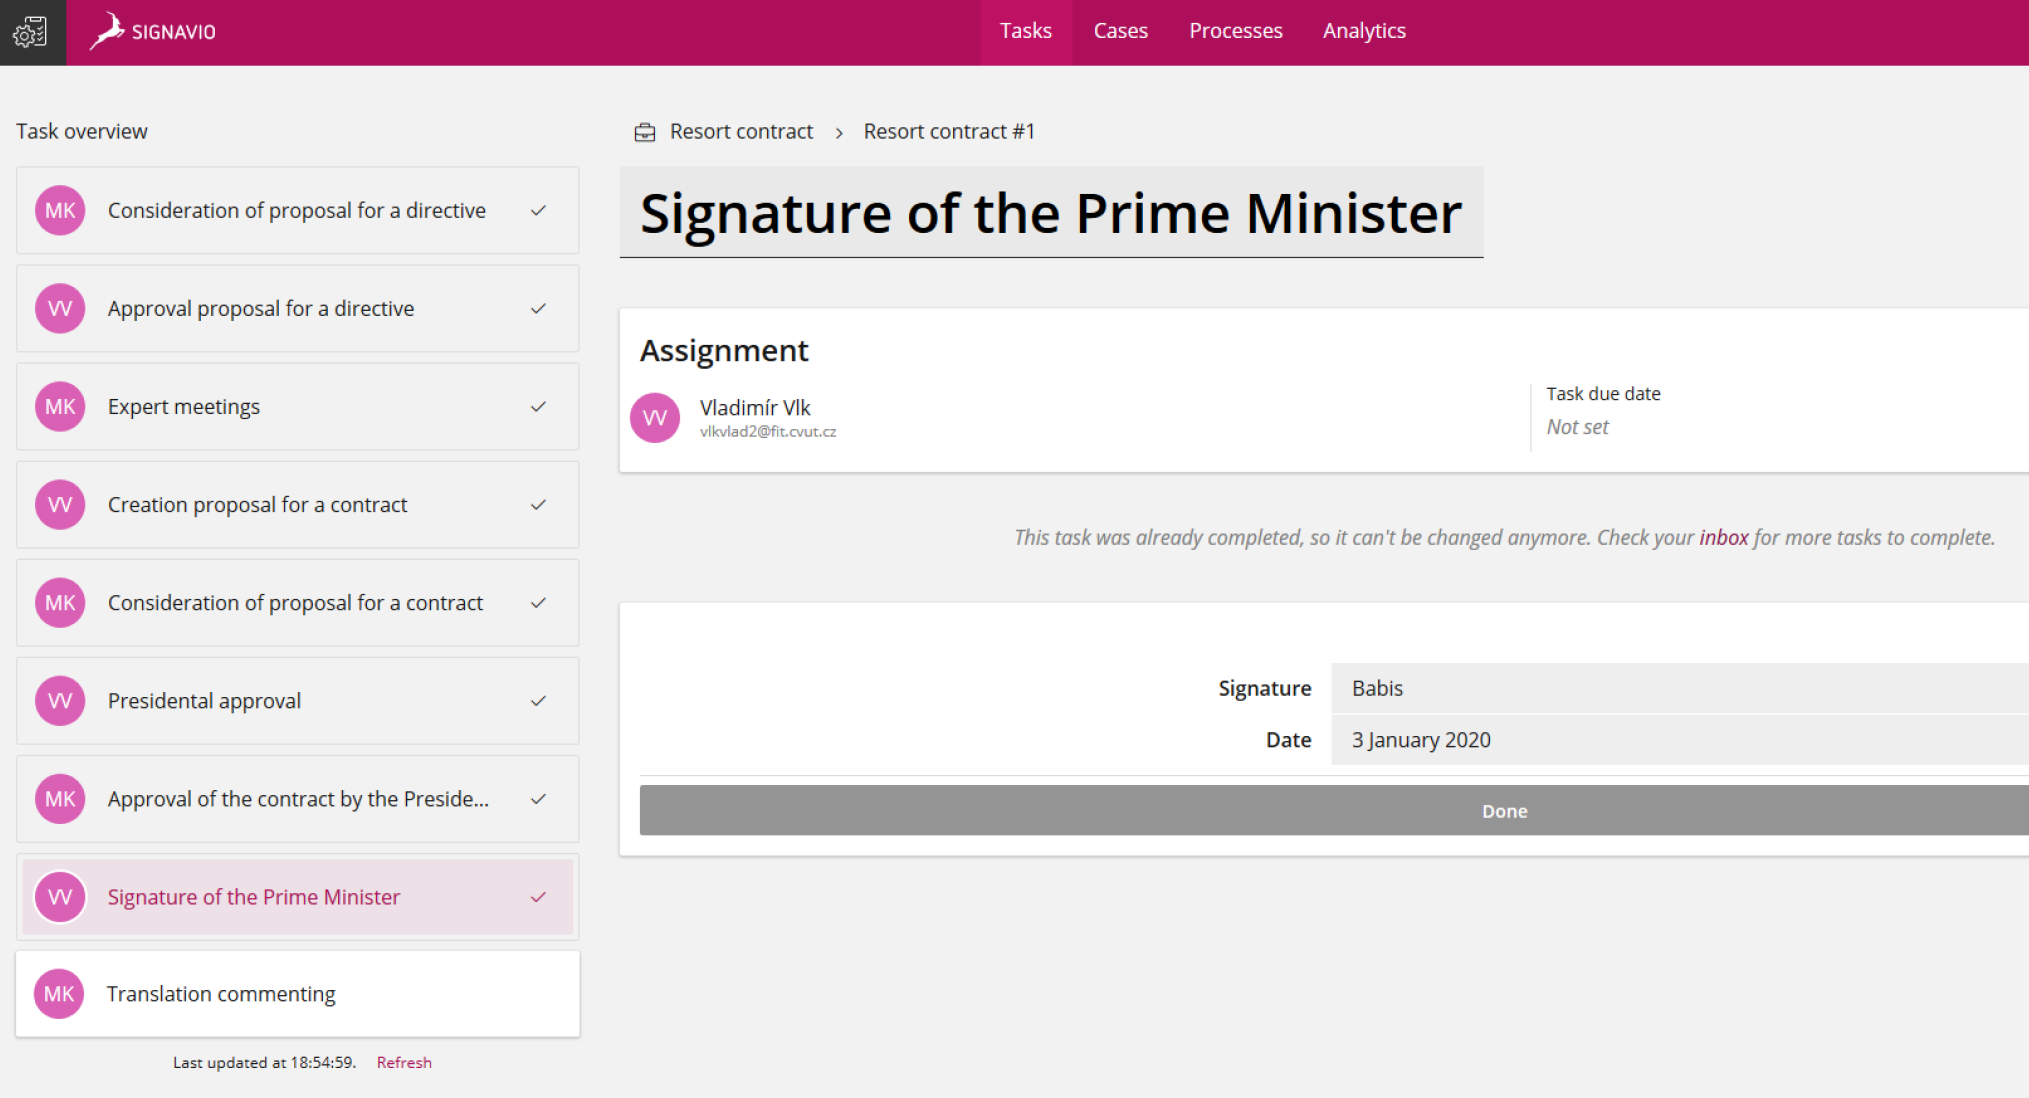
\includegraphics[width=\textwidth]{pic/BPMNExecution2}
	\caption{A BPMN Process Execution~\cite{kutisvlk2019}}
	\label{fig:bpmnExecution2}
\end{figure}

\section{Process Analytics}

\begin{figure}[h]\centering
	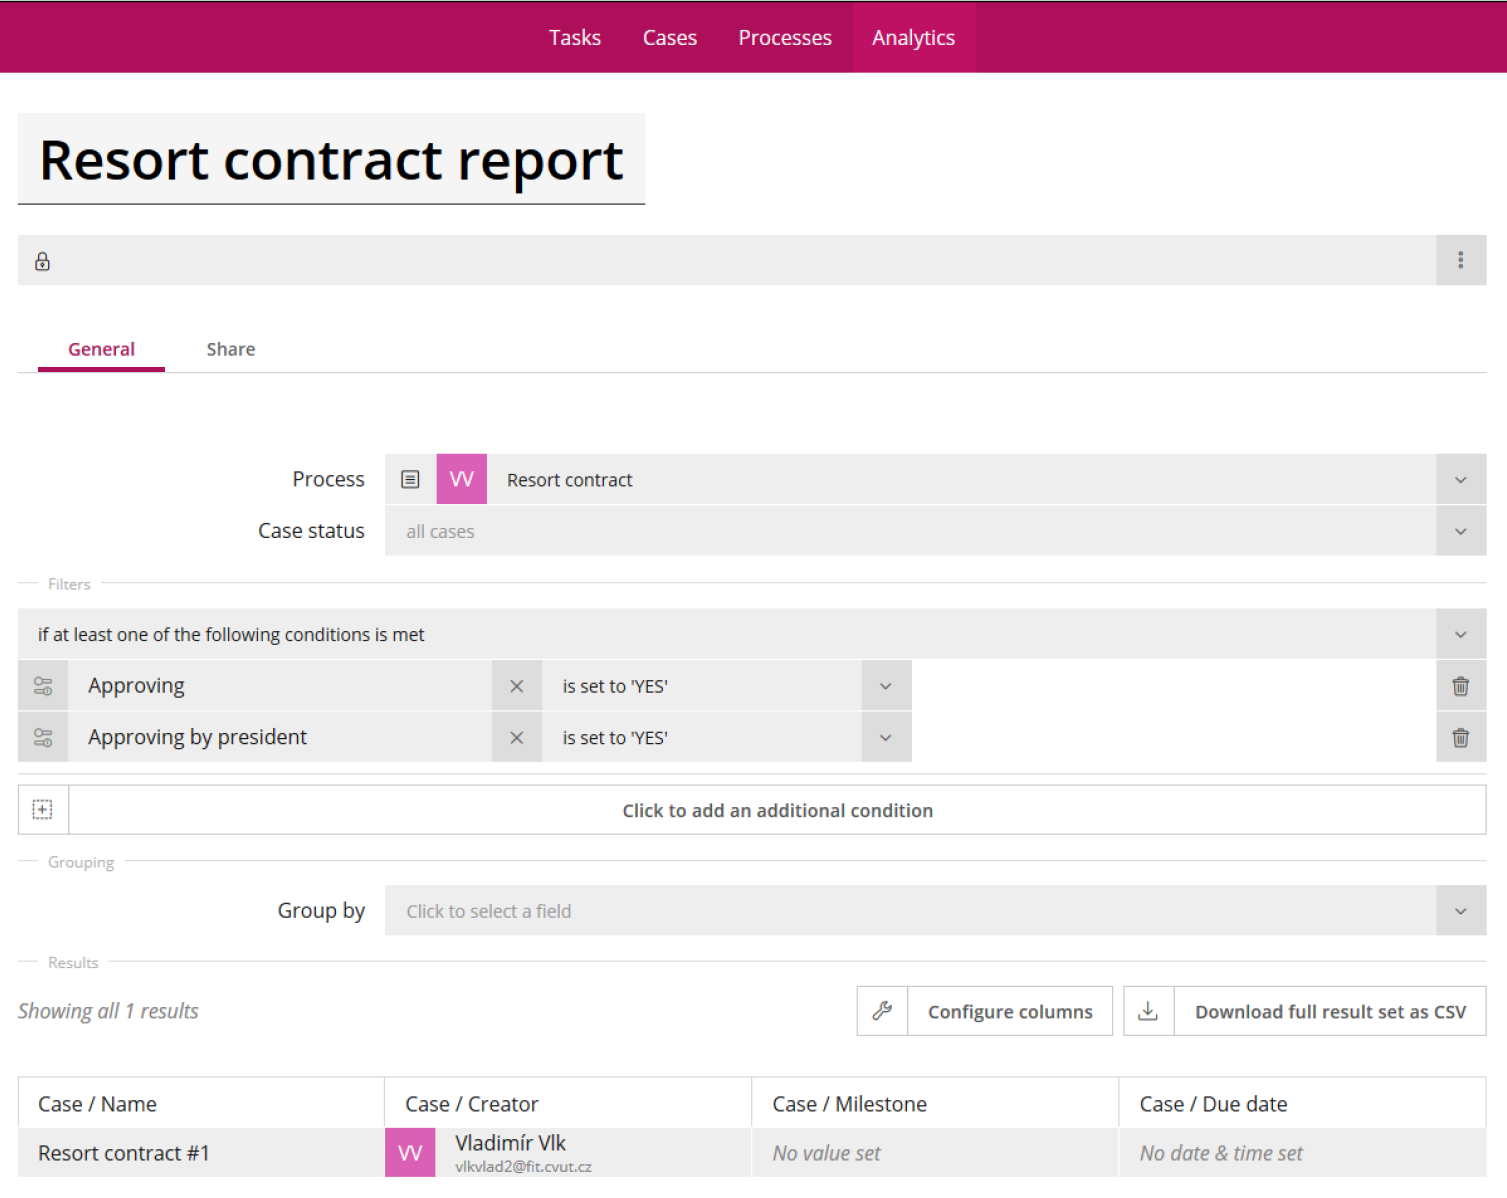
\includegraphics[width=\textwidth]{pic/BPMNReport}
	\caption{A BPMN Process Report~\cite{kutisvlk2019}}
	\label{fig:bpmnReport}
\end{figure}

\section{Results Presentation}\label{sec:presentation}

An url to your 2 min presentation where you present an executive level summary of your efforts. Imagine you are presenting it to a customer who paid 100k EUR for the work. \url{https://www.youtube.com/watch?v=qfprck_Djro} 